\subsection{Preemptible functions: \textit{libinger}}
\label{sec:libinger}

The libinger library implements the preemptible function interface.
To provide an API centered around familiar function calls that adhere to the standard
stack discipline, the library hides internal unstructured control flow.
When \texttt{launch()} and \texttt{resume()} are executing the user-provided
function, they use a signal handler to asynchronously monitor its execution.  If
it exceeds its timeout, libinger must jump back to the caller, returning a
continuation that stores the preemptible function's register values.
Because the continuation might later be resumed, \texttt{launch()} cannot allow the
caller's intervening code to clobber the stack frames left behind by preemption, and
must therefore invoke the user function on a separate execution stack.  The library
implements all of these steps in userland.

Although seeking to implement low-latency preemption without requiring a custom
operating system, we sought a design that could operate with performance comparable
to Shinjuku's.  Our prototype is not yet optimized to this extent, but
we provide a back of the envelope calculation of its minimum possible preemption
latency based on Shinjuku's
comparison of the latency of bare-metal interprocessor interrupts (IPIs)
versus Linux signals (measured from their request by one core to the
invocation of the other's interrupt service routine or signal handler).  While
IPIs take an average of only 1993 cycles, compared to 4950 for
signals (a ratio of 1:2.5), a look at their sender/receiver breakdown of the latter
number suggests two opportunities to reduce this overhead without
abandoning the existing systems software stack:  First, 343 of those cycles (6.9\%)
are spent propagating the signal between the two cores, and should largely disappear
by initiating it on the same thread that is to be preempted.  Second, 2084 cycles
(42\%) are incurred by the sender, of which some portion should also
disappear~\cite{Kaffes:nsdi2019}.  We therefore expect that an optimized system based
on intra-thread signals built atop the existing system stack could achieve an
average preemption latency within 2.5x of that of their custom operating
system with a dedicated watchdog core.

Before jumping into a preemptible function, libinger enables preemption by
configuring a per-thread POSIX timer to periodically invoke a signal handler on the
current thread.  Unfortunately, when a multithreaded application receives a signal,
the kernel delivers it to an arbitrary thread~\cite{signal-manpage}.  We work around
this limitation by allocating a separate preemption signal for each thread that is
currently invoking a preemptible function:  Each threads use the same handler, but
stores its signal numbers in a thread-local variable.  Whenever the handler runs, it
checks whether it was triggered by the current thread's signal.  If not, it masks the
rogue signal and immediately returns; in this way, the system quickly converges to
delivering each preemption signal only to its corresponding thread.  The current
implementation sets each timer to fire at a fixed scheduling interval in the tens of
microseconds\footnote{The efficiency of long-running preemptible functions could be
improved by delaying the start of these periodic signals until
hundreds of microseconds before the timeout was hit; in this way, most of long
functions' execution time would run without any throughput degradation, yet their
preemption could still be quite accurate (free of warmup effects).}.  Compared to the
preemption mechanism from RT, our saves a level of signal indirection by eliminating
their central watchdog thread that received all timer signals and forwarded them to
workers using \texttt{pthread\_kill()}.

Figure~\ref{fig:callsimple} shows what happens on each call to \texttt{launch()}.
We create a \textbf{checkpoint} continuation using the POSIX
\texttt{getcontext()} function~\cite{getcontext-manpage}; this will be needed if the
preemptible
function times out.  Next, we allocate a fixed-size execution stack and switch to it
using the \texttt{makecontext()} and \texttt{setcontext()} functions.  Then, if the
current thread doesn't already have a preemption signal assigned, we allocate one
from a pool of unused signal numbers\footnote{While it would be straightforward to
track which signals the application used by intercepting its calls to
\texttt{signal()} and \texttt{sigaction()}, we haven't yet implemented this in our
prototype:\@ instead, it uses a pool of rarely-used signals that may conflict with
some programs.}.  Finally, we configure a POSIX timer via
\texttt{timer\_settime()} and call the user-provided preemptible funcion.

\begin{figure}
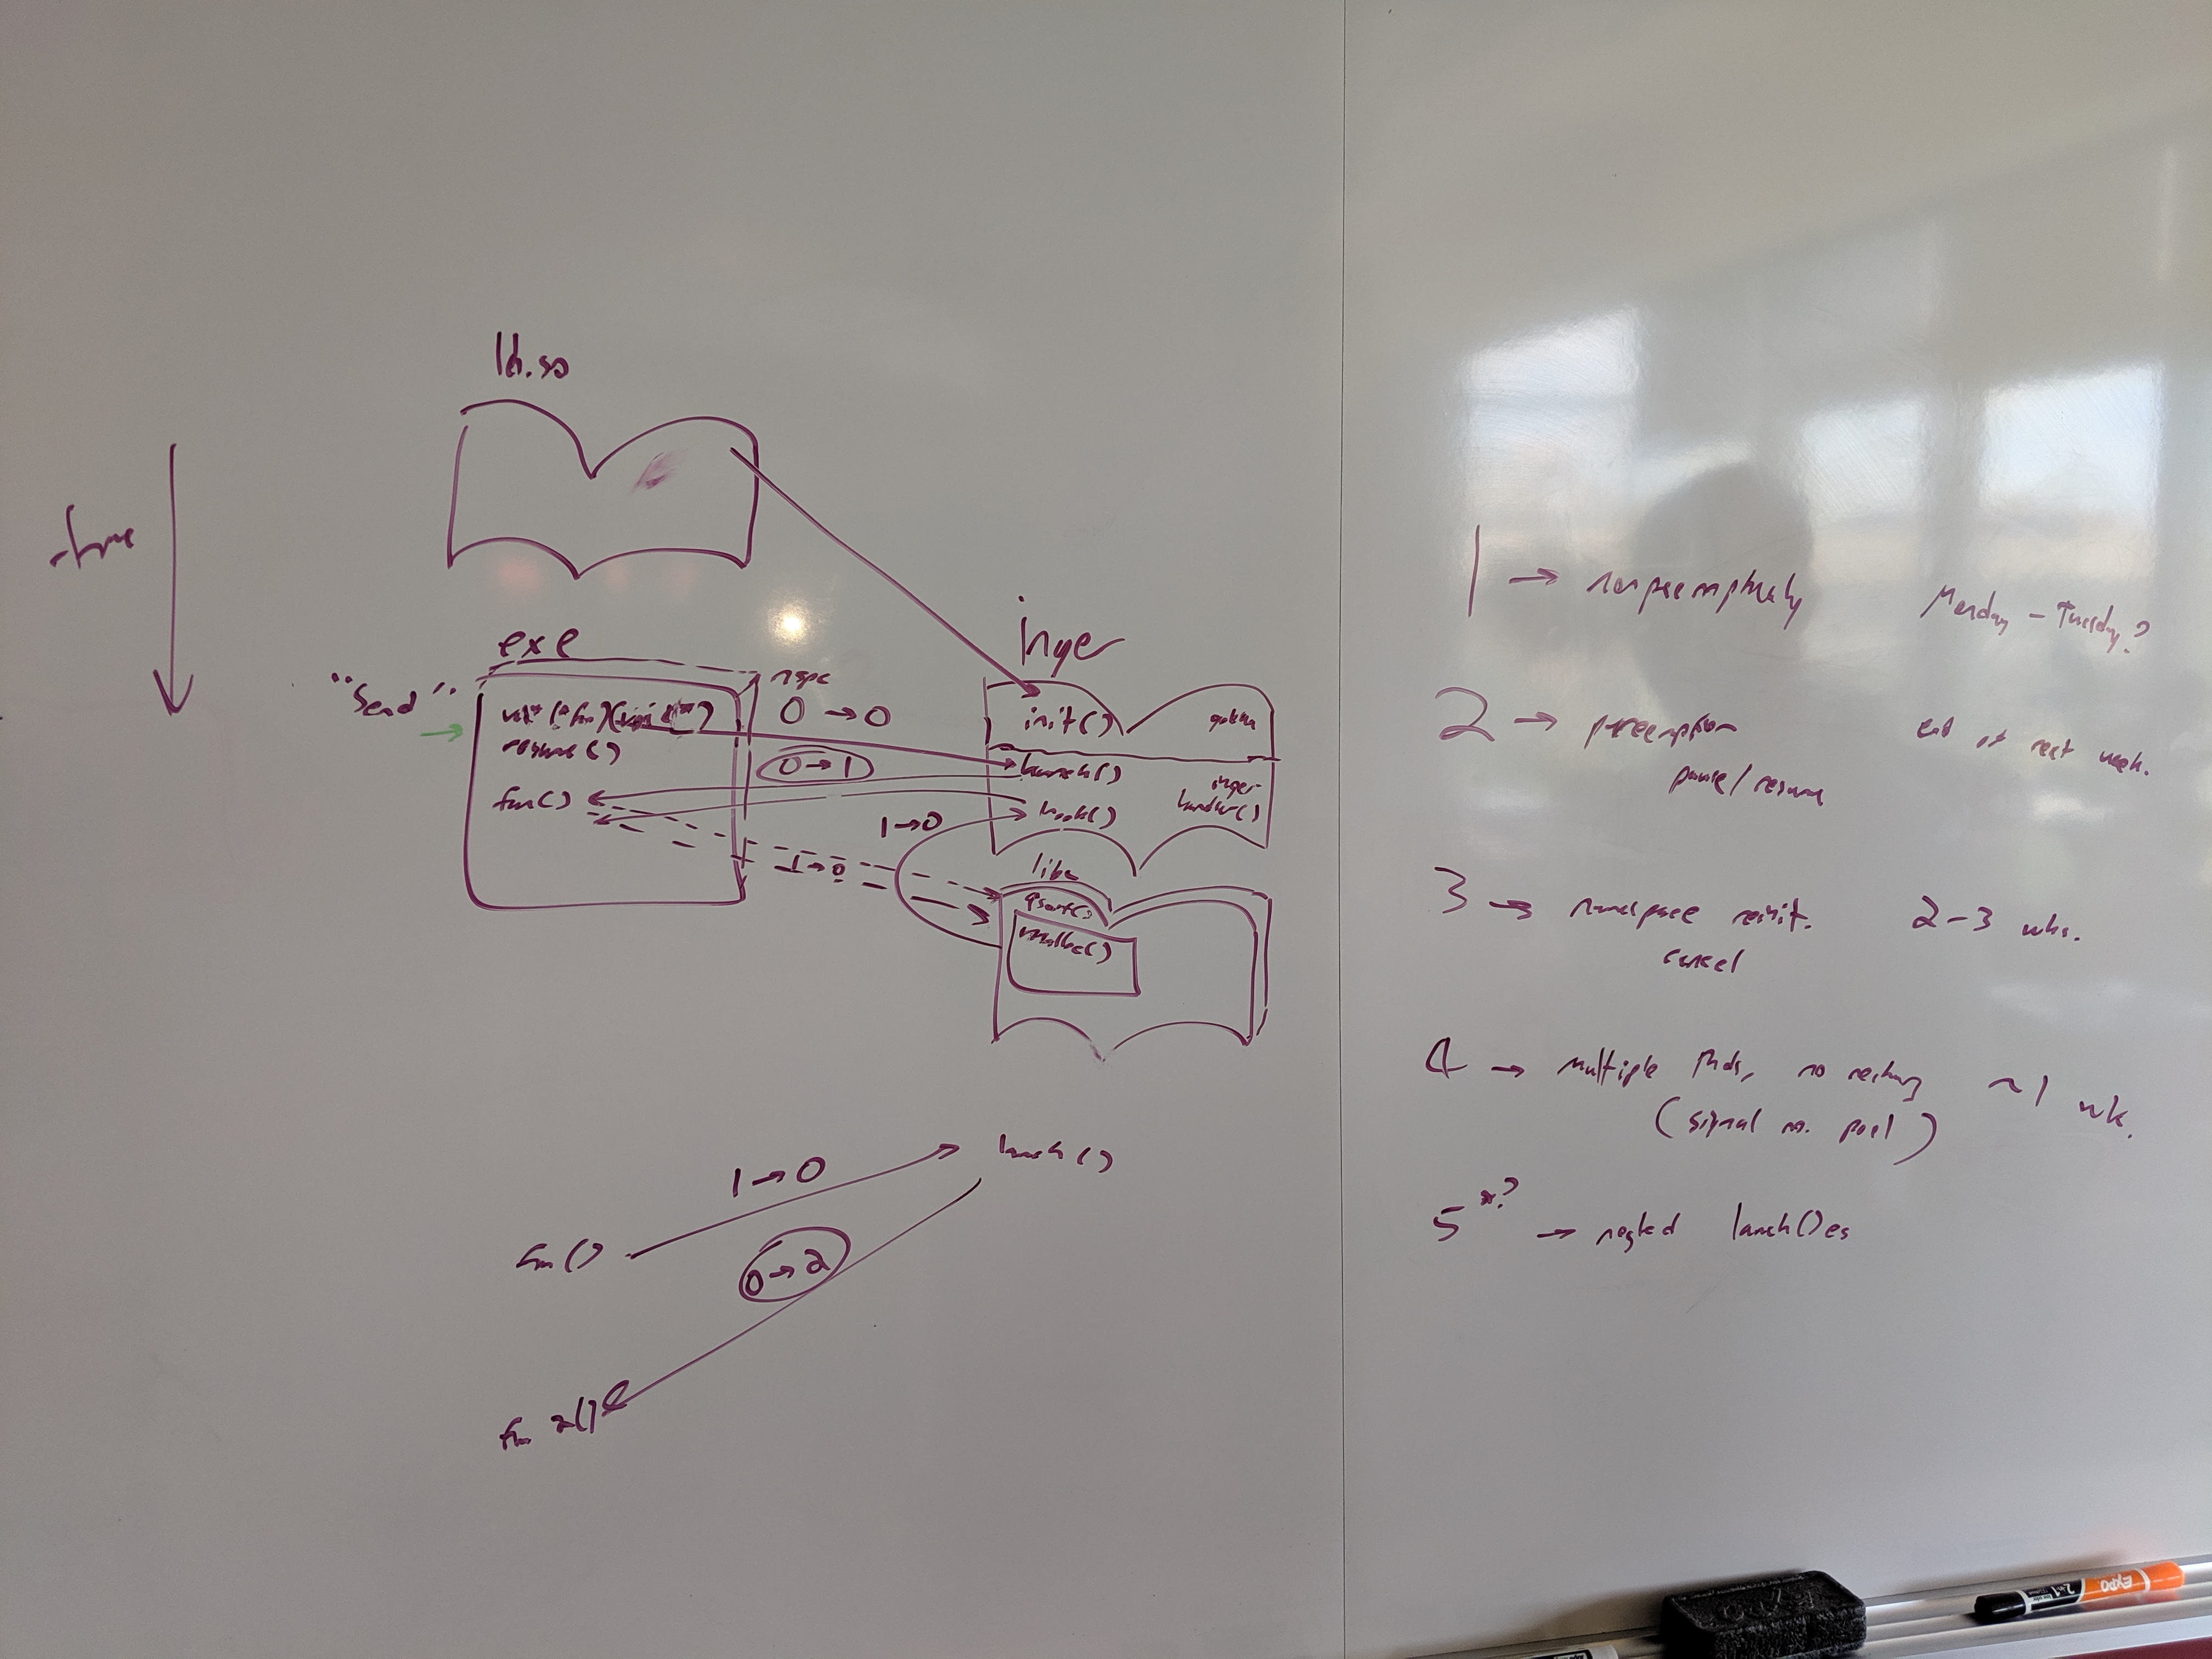
\includegraphics[width=\columnwidth]{figs/calltree}
\caption{Preemptible function dispatch}
\label{fig:callsimple}
\end{figure}

While the preemptible function is running, the POSIX timer fires periodically,
causing a signal handler to be invoked each time.  Figure~\ref{fig:twostacks} shows
the two stacks of execution present while the handler is running, as well as what
happens to the stack frames of both if the function times out.  The handler first
checks whether the preemption signal was intended for the current thread, as
described earlier.  It then checks whether the preemptible function has exceeded its
timeout; if so, it swaps the contents of the signal handler's continuation
(accessible via the final argument to the function~\cite{sigaction-manpage}) with the
checkpoint continuation saved by \texttt{launch()}.  This causes the subsequent
return from the signal handler to jump back to \texttt{launch()}, which then returns
a \texttt{linger} structure containing the signal handler's original context.  A
subsequent \texttt{resume()} call on this packaged continuation proceeds in much the
same way as \texttt{launch()}, but resumes the original computation by sending itself
a special signal with \texttt{pthread\_kill()}, then swapping the saved context with
the contents of that handler's context\footnote{This is necessary because POSIX left
the semantics of calling \texttt{setcontext()} on the continuation saved by a signal
handler invocation unspecified, leading implementations such as GNU not to handle
this case~\cite{getcontext-manpage}.}.

\begin{figure}
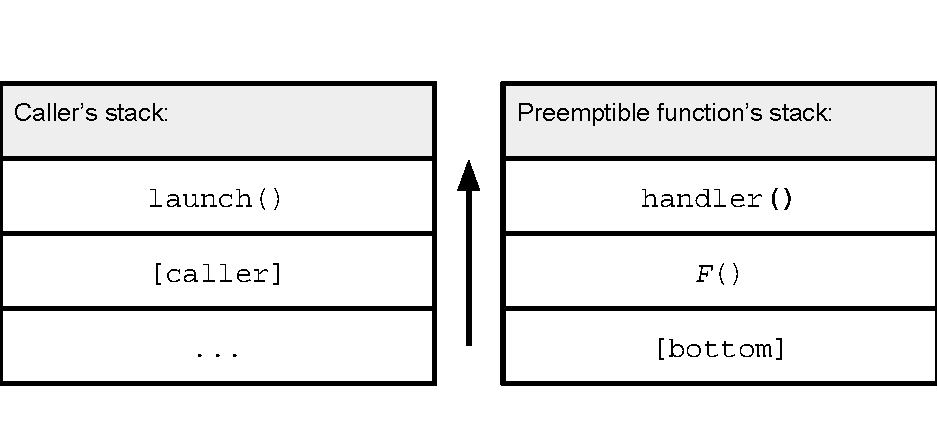
\includegraphics[width=\columnwidth]{figs/twostacks}
\caption{The stacks before and after a timeout.  \textnormal{Upon discovering
that the preemptible function has exceeded its time bound, the handler returns to the
checkpoint continuation within the \texttt{launch()} function, removing its own stack
frame in the process.  Then, \texttt{launch()} returns to the original call site,
which removes its stack frame.}}
\label{fig:twostacks}
\end{figure}

When the caller is finished with a preemptible function, it must deallocate it either
explicitly (C) or implicitly via the \texttt{inger} type's destructor (Rust).  This
cleans up the libinger resources allocated by \texttt{launch()}; however, if the call
constitutes a cancellation, the current implementation of libinger does not
automatically clean up resources already allocated by the preemptible function
itself.  While the lack of a standard deinitialization API makes this inherently hard
to do in C, it is possible to implement in languages such as Rust that support
destructors.  For instance, the approach proposed by Boucher et
al.~\cite{boucher:atc2018} could be employed to raise a panic (exception) on the
preemptible function's stack, causing the language runtime to unwind each stack frame,
invoking the destructor of each local variable in the process.

\subsection{Case study: Userland threading}
\label{sec:threading}
